

\documentclass[twoside,twocolumn]{article}

\usepackage{blindtext} % Package to generate dummy text throughout this template 
\usepackage{graphicx}
\usepackage[sc]{mathpazo} % Use the Palatino font
\usepackage[T1]{fontenc} % Use 8-bit encoding that has 256 glyphs
\linespread{1.05} % Line spacing - Palatino needs more space between lines
\usepackage{microtype} % Slightly tweak font spacing for aesthetics

\usepackage[spanish]{babel} % Language hyphenation and typographical rules

\usepackage[hmarginratio=1:1,top=32mm,columnsep=20pt]{geometry} % Document margins
\usepackage[hang, small,labelfont=bf,up,textfont=it,up]{caption} % Custom captions under/above floats in tables or figures
\usepackage{booktabs} % Horizontal rules in tables

\usepackage{lettrine} % The lettrine is the first enlarged letter at the beginning of the text

\usepackage{enumitem} % Customized lists
\setlist[itemize]{noitemsep} % Make itemize lists more compact

\usepackage{abstract} % Allows abstract customization
\renewcommand{\abstractnamefont}{\normalfont\bfseries} % Set the "Abstract" text to bold
\renewcommand{\abstracttextfont}{\normalfont\small\itshape} % Set the abstract itself to small italic text

\usepackage{titlesec} % Allows customization of titles
\renewcommand\thesection{\Roman{section}} % Roman numerals for the sections
\renewcommand\thesubsection{\roman{subsection}} % roman numerals for subsections
\titleformat{\section}[block]{\large\scshape\centering}{\thesection.}{1em}{} % Change the look of the section titles
\titleformat{\subsection}[block]{\large}{\thesubsection.}{1em}{} % Change the look of the section titles

\usepackage{fancyhdr} % Headers and footers
\pagestyle{fancy} % All pages have headers and footers
\fancyhead{} % Blank out the default header
\fancyfoot{} % Blank out the default footer
\fancyhead[C]{Las nuevas características del estándar SQL:2011 $\bullet$ Agosto 2019 $\bullet$ } % Custom header text
\fancyfoot[RO,LE]{\thepage} % Custom footer text

\usepackage{titling} % Customizing the title section

\usepackage{hyperref} % For hyperlinks in the PDF

%----------------------------------------------------------------------------------------
%	TITLE SECTION
%----------------------------------------------------------------------------------------

\setlength{\droptitle}{-4\baselineskip} % Move the title up

\pretitle{\begin{center}\Huge\bfseries} % Article title formatting
\posttitle{\end{center}} % Article title closing formatting
\title{La nuevas características de el estándar SQL:2011} % Article title
\author{Sigfredo Aponte Roldán}
\date{\today} % Leave empty to omit a date
\renewcommand{\maketitlehookd}{%
\begin{abstract}
\noindent 
This article explains and describes the new features of ISO / IEC 9075: 2011 or SQL: 2011, which is the seventh revision of the ISO and ANSI standard for the query language of the SQL database. The standard consists of 9 parts that are described in detail.
\end{abstract}
\begin{abstract}
\noindent 
En el presente artículo se explica y describen las nuevas características de el ISO/IEC 9075:2011 o SQL:2011, el cual es la séptima revisión del estándar ISO y ANSI para el lenguaje de consulta de la base de datos SQL. El estándar consta de 9 partes que se describen en detalle.
\end{abstract}
}

%----------------------------------------------------------------------------------------

\begin{document}

% Print the title
\maketitle

%----------------------------------------------------------------------------------------
%	ARTICLE CONTENTS
%----------------------------------------------------------------------------------------

\section{Introduccion}
\lettrine[nindent=0em,lines=3]{S}QL es el estandar publicado e introducido por ISO(International Organization for Standardization) y IEC(International Electrotechnical Commission). En diciembre del 2011, ISO/IEC publico la ultima edicion de SQL, SQL:2011.
El estándar SQL es publicado en múltiples volúmenes, llamado partes. Este estándar consta de nueve partes, numeradas 1, 2, 3, 4, 9, 10, 11, 13 y 14. Por mucho la parte mas importante en la parte 2, que a su vez es la mas larga con 1470 paginas(casi 100 paginas mas que en el SQL:2008). Solo cinco partes son revisadas en el SQL:2011; para las otras cuatro partes, la version publicada en SQL:2008 permanece vigente. En este articulo nos concentraremos en las nuevas características que se encuentras en SQL:2011. El estandar SQL especifica caracteristicas opcionales y obligatorias. Las caracteristicas obliigatorias no son cambiadas desde SQL:1999. Quizas las nuevas caracteristicas mas importantes del SQL:2011 estan en el area del de las base de datos temporales. Las mas importantes caracteristicas del SQL:2011 que se trataran son las siguientes:
\begin{itemize}
\item DELETE in MERGE.
\item Canalizado DML.
\item Mejoras CALL.
\item Capacidad de busqueda limitada.
\item Restricciones de tablas no forzadas.

\end{itemize}


%------------------------------------------------

\section{Marco Teórico}

\subsection{Bases de Datos Relacionales}

Una base de datos es relacional cuando esta cumple con el modelo relacional, que se refiere a la relación que existe entre las distintas entidades o tablas de la base. También conocidas como sistemas de gestión de bases de datos relacionales (RDBMS), las cuales nos permiten almacenar y gestionar gran cantidad de datos. Los datos se almacenan en diferentes tablas y las relaciones se establecen usando claves primarias u otras llaves conocidas como claves externas o foráneas.

Existen un sinnúmero de sistemas de gestión de bases de datos relacionales y cada una de ellas posee una forma diferente de manejar su data, algunos ejemplos de RDBMS son: Oracle, MySQL, SQL Server, entre otras.
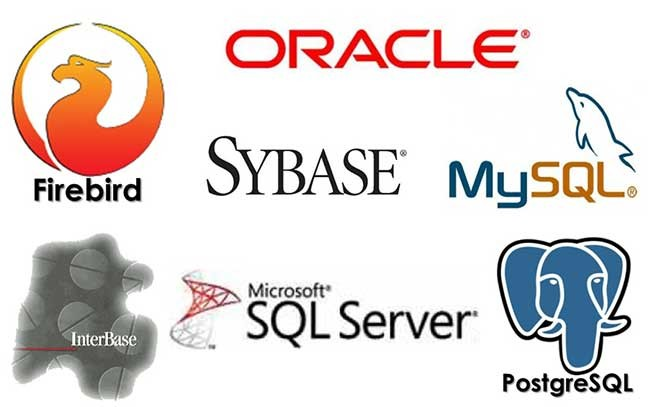
\includegraphics[width=7cm]{./Imagenes/sistemasgestionbd} 
\subsection{SQL}

SQL es un lenguaje estándar e interactivo de acceso a base de datos relacionales que permite especificar diversos tipos de operaciones en ella, gracias a la utilización del álgebra y de cálculos relaciones. el SQL brinda la posibilidad de realizar consultas con el objetivo de recuperar información de las bases de datos de manera sencilla.

\includegraphics[width=7cm]{./Imagenes/sql}  

\subsection{¿Por qué aprender SQL?}

SQL es un lenguaje declarativo estándar internacional de comunicación dentro de las bases de datos que nos permite a todos el acceso y manipulación de datos en una base de datos, y además se puede integrar a lenguajes de programación, por ejemplo ASP o PHP, y en combinación con cualquier base de datos específica, por ejemplo MySQL, SQL Server, MS Access, entre otras.
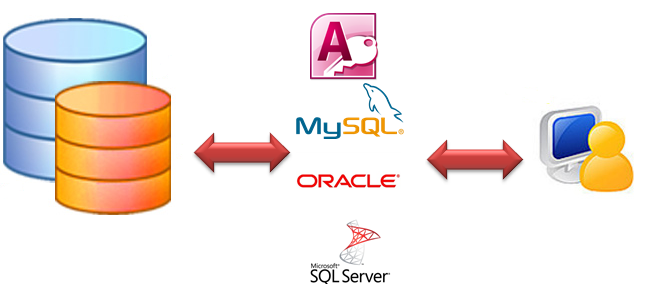
\includegraphics[width=7cm]{./Imagenes/basedatossql} 

%------------------------------------------------

\section{Análisis}
En la siguiente sección empezaremos a analizar y ver las nuevas características que nos trae el estándar SQL:2011, mencionadas anteriormente en la introducción.

\subsection{DELETE in MERGE}
MERGE es una manipulación de datos introducida en SQL:2003 y mejorada en SQL:2008. Aquí analizaremos un ejemplo que es permitido por SQL:2008. Suponiendo que "Inventario (Parte, Cantidad)" es una tabla que lista partes y cantidad, y "Cambios (Parte, Cantidad, Accion)" es una tabla de cambios que serán aplicados a la tabla Inventario. La columna Accion tiene dos valores, con las siguiente connotación:
\begin{itemize}
\item 'Mod': Añade de la tabla Cambios(Cantidad) a la tabla Inventario(Cantidad) si la columna parte existe en la tabla inventario.
\item 'Nuevo': Añade una nueva fila a la tabla Inventario usando los valores de la columna Parte de la tabla Cambio y la columna cantidad de la tabla Cambio.
\end{itemize}
En el SQL:2008 esto seria posible usando el siguiente código.
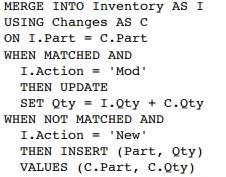
\includegraphics[width=7cm]{./Imagenes/codigo1} 
Ahora esto cambio en el SQL:2011 ya que se a añadido una nueva habilidad para realizar DELETE sin el comando MERGE. Esto se realizaria con el siguiente código.
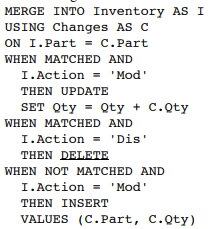
\includegraphics[width=7cm]{./Imagenes/codigo2} 
\subsection{Canalizado DML}
El canalizado DML añade una opcion para realizar coando de cambios de datros(INSERT,UPDATE,DELETE,MERGE) sin seleccionar el comando.
Un comando de cambio de datos tiene una o dos tablas que contienen filas especificas que seran alteradas. El Canalizado DML probee acceso a toda la informacion antigua de la tabla o nueva informacion sin seleccionarla utilizando el comando SELECT. Por ejemplo.
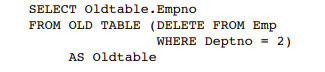
\includegraphics[width=7cm]{./Imagenes/codigo3} 
\subsection{Mejoras CALL}
El metodo CALL fue introducido en la Parte 4 PSM en 1996 y luego incorporado posteriormente en la Parte 2 del SQL:1999 y es usado para invocar algun metodo SQL. Aqui veremos un ejemplo de como se llama un metodo en el estandar SQL:2011.
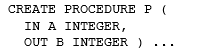
\includegraphics[width=7cm]{./Imagenes/codigo4} 
\subsection{Capacidad de busqueda limitada}
Una tarea utilizada muy comunmente es el de buscar filas en una tabla y el limitar el número de resultados. Por ejemplo solo mostrar los 10 primeros resultados de una busqueda. Un ejemplo de esto soportado por el estandar SQL:2008 sería:
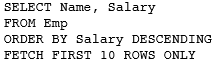
\includegraphics[width=7cm]{./Imagenes/codigo5}
En el estandar SQL:2011 esta sintaxis cambia en algunas cosas. Por ejemplo en el siguiente codigo mostraremos como seria la manera correcta de ejecutar este comando con el estandar SQL:2011.
 
\includegraphics[width=7cm]{./Imagenes/codigo6}
 En este estandar se remplazaria la palabra subrayada WITH TIES con el comando ONLY como se ve en el siguiente ejemplo:
  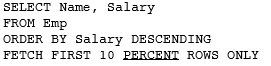
\includegraphics[width=7cm]{./Imagenes/codigo7}
\subsection{Restricciones de tablas no forzadas}
Las constraints de las tablas son declaradas en los posibles valores de las filas de una tabla. Existen tres tipos: Restricciones Unicas(requieren el valor de una columna o un conjunto de columnas).
Bajo la mayoria de circunstancias, el usuario desea que las restricciones sean forzadas, desde que son vitales para el matenimiento de la intgridad de los datos. En tal caso, hay situaciones en los que los usuqario desean temporalmente borrar o deshabilitar estas restricciones. SQL:2011 añadió una solución a este problema, añadiendo una sintaxis apara laterar la restriccion para que esta no sea forzada.


\section{Conclusiones}
Los estandares cada vez se hacen mas y mas indispensables para el desarrollo de cualquier producto tecnologico, y mas en el caso de una base de datos en donde toda la informacion debe estar estructurada de tal manera en la que todos los usuarios que tengan acceso a esta, logren entender y puedan interactuar con esta de eficientemente,debido a esto, es sumamente importante mantenernos al dia con las diferentes caracteristicas nuevas que se añaden año tras año, con las nuevas ediciones que se dan de los estandares SQL, ya que de esta manera podemos optimizary agilizar nuestro trabajo a la par que facilitar el entendimiento de los usuarios de la base de datos.
%	REFERENCE LIST
%----------------------------------------------------------------------------------------

\begin{thebibliography}{99} % Bibliography - this is intentionally simple in this template
\bibitem[Codina, 2015]{Luis Codina:2015dg}
Codina, L (2015).
\newblock Sistemas gestion de bases de datos documentales.


\bibitem[1]{ISO/IEC 9075-1_2011}
Information technology-Databse lenguages-SQL-Part1:Framework (2011).

\bibitem[2]{ISO/IEC 9075-1_2011}
Information technology-Databse lenguages-SQL-Part2:Foundation(SQL/Foundation)(2011).

\bibitem[3]{ISO/IEC 9075-1_2011}
Information technology-Databse lenguages-SQL-Part3:Call-Level Interface(2011).

\bibitem[4]{ISO/IEC 9075-1_2011}
Information technology-Databse lenguages-SQL-Part4:Persistent Stred Modules(SQL/PSM) (2011).

\bibitem[5]{ISO/IEC 9075-1_2011}
Information technology-Databse lenguages-SQL-Part9:Managment of External Data(SQL/MED)(2011).

 
 
\end{thebibliography}

%----------------------------------------------------------------------------------------

\end{document}
